%% Based upon `elsarticle-template-3-num.tex',
\documentclass[preprint,12pt]{elsarticle}
%%\documentclass[final, 5p, times, twocolumn]{elsarticle}

\usepackage{epsfig} %for TEXworks on Windows 7

%% if you use PostScript figures in your article
%% use the graphics package for simple commands
%% \usepackage{graphics}
%% or use the graphicx package for more complicated commands
%% \usepackage{graphicx}
%% or use the epsfig package if you prefer to use the old commands
%%\usepackage{epsfig}
\usepackage{algorithm,algorithmic, graphicx, natbib, amsmath, subfigure} 

%% The amssymb package provides various useful mathematical symbols
\usepackage{amssymb}
%% The amsthm package provides extended theorem environments
%% \usepackage{amsthm}

%% The numcompress package shorten the last page in references.
%% `nodots' option removes dots from firstnames in references.
\usepackage[nodots]{numcompress}

%% The lineno packages adds line numbers. Start line numbering with
%% \begin{linenumbers}, end it with \end{linenumbers}. Or switch it on
%% for the whole article with \linenumbers after \end{frontmatter}.
%% \usepackage{lineno}

%% natbib.sty is loaded by default. However, natbib options can be
%% provided with \biboptions{...} command. Following options are
%% valid:

%%   round  -  round parentheses are used (default)
%%   square -  square brackets are used   [option]
%%   curly  -  curly braces are used      {option}
%%   angle  -  angle brackets are used    <option>
%%   semicolon  -  multiple citations separated by semi-colon
%%   colon  - same as semicolon, an earlier confusion
%%   comma  -  separated by comma
%%   numbers-  selects numerical citations
%%   super  -  numerical citations as superscripts
%%   sort   -  sorts multiple citations according to order in ref. list
%%   sort&compress   -  like sort, but also compresses numerical citations
%%   compress - compresses without sorting
%%
%% \biboptions{comma,round}

% \biboptions{}


\journal{Communications in Nonlinear Science and Numerical Simulation}

\begin{document}

\begin{frontmatter}

%% Title, authors and addresses

%% use the tnoteref command within \title for footnotes;
%% use the tnotetext command for the associated footnote;
%% use the fnref command within \author or \address for footnotes;
%% use the fntext command for the associated footnote;
%% use the corref command within \author for corresponding author footnotes;
%% use the cortext command for the associated footnote;
%% use the ead command for the email address,
%% and the form \ead[url] for the home page:
%%
%% \title{Title\tnoteref{label1}}
%% \tnotetext[label1]{}
%% \author{Name\corref{cor1}\fnref{label2}}
%% \ead{email address}
%% \ead[url]{home page}
%% \fntext[label2]{}
%% \cortext[cor1]{}
%% \address{Address\fnref{label3}}
%% \fntext[label3]{}

\title{An efficient broadband deep memory algorithm for computing fractional order operators}

%% use optional labels to link authors explicitly to addresses:
%% \author[label1,label2]{<author name>}
%% \address[label1]{<address>}
%% \address[label2]{<address>}

\author[Dorsher]{Steven Dorsher\footnote{Corresponding author}\footnote{Mailing address: 3152 Blackheath Drive, Saint Cloud, Minnesota 56301}}
\author[Bohannan]{Gary Bohannan}

\address[Dorsher]{Department of Chemistry and Physics, Saint Cloud State
  University \\
720 4th Avenue South, WSB 324, Saint Cloud, Minnesota, 56301, USA\\
1-952-686-1925\\
sdorsher@gmail.com}

\address[Bohannan]{Department of Chemistry and Physics, Saint Cloud State
  University \\
720 4th Avenue South, WSB 324, Saint Cloud, Minnesota, 56301, USA\\
gwbohannan@stcloudstate.edu}

 \begin{abstract}

This paper outlines a method to achieve effective bandwidth of five or
more decades in the approximation of a fractional order
derivative. This constitutes an increase of two decades or more in 
constant-phase bandwidth (to within $10^\circ$ of phase ripple) over
current algorithms, such the Infinite Impulse Response (IIR) method
based on continued fraction expansion, while demanding only slightly
more computational steps and processor memory.

\end{abstract}

\begin{keyword}
fractional calculus \sep numerical methods \sep computational efficiency

\MSC[2010] 65Y02 \sep 65Z02 \sep 65Y04 \sep 65Z04
\end{keyword}

\end{frontmatter}

%%\footnote{IIR -- Infinite Impulse Response\\
%%FO -- Fractional Order\\
%%GL --  Full Gr{\"u}nwald calculation\\ {  }GL\# -- Truncated Gr{\"u}nwald calculation to \# terms\\
%%LIN\# -- Linear binning, \# bins\\
%%SQ\# -- Squared binning, \# bins\\
%%EXP\# -- Exponential binning with a base of two, \# bins\\
%%FIB\#-- Fibonacci binning, \# bins}

%%
%% Start line numbering here if you want
%%
% \linenumbers

%% main text

\section{Introduction}\label{sec:intro}
\setcounter{section}{1}
\setcounter{equation}{0}

Interest in the application of the fractional calculus has been
growing at an ever increasing rate. Of long term and continued
interest is in the use of fractional order (FO) operators, such as
integrators and differentiators, in motion control
applications.~\cite{Luo:13} While wide bandwidth analog controllers
have been successfully demonstrated~\cite{Bohannan:08}, fractional
order analog circuit elements are not generally available and the
prototypes that have been demonstrated do not have the ability to be
retuned for a specific desired phase.~\cite{Monje:10}

Unfortunately, the existing techniques for digital approximation of FO
operators are limited in bandwidth to on the order of three and a half
decades of frequency response while nonlinear effects in motion
control systems can span five decades or more. This places a severe
constraint on the design and implementation of digital FO controllers,
i.e. how to set the sampling frequency to meet the high speed
requirements necessitated by the Nyquist sampling rate while at the
same time providing enough deep memory to get low offset
error. Additionally, the infinite impulse response type of
implementation cannot guarantee stability due to the limitations of
finite precision arithmetic. See e.g.~\cite{Chen:04a}.

Given the current necessity to implement FO controls in digital form,
it is desirable to obtain the most efficient algorithm to compute a
fractional order operator while maximizing the numerical stability of
the algorithm. Efficiency to be measured in both memory utilization
and number of computations per time step. This paper outlines a
computational method inspired by the Riemann-Liouville integral
definition and the Gr{\"u}nwald algorithm.~\cite{OldSpan:74} The
essential concept is the rescaling of time by successive accumulation
of older data into increasing size bins for deeper memory.




\paragraph{Outline\\}
We will first describe a novel approach based on successive 
binning of older data and resource requirements for the 
algorithm, then we will compare the results with other
approaches.

%in Comm. in Nonlin. Sci. and Num. Sim. language, 
%introduction=introduction
%algorithmDefn=theory
%computation=calculation
%methods = verification methods. logically follows theory, but is a methods section
%bode=results
%conclusions=conclusions

\begin{itemize} 
\item Section~\ref{sec:algorithmDefn} contains the definition of
the algorithm. 
\item  Section~\ref{sec:computation} provides an analysis of the
  computational resources required for the larger versus the smaller
  number of memory registers required.
\item Section~\ref{sec:methods} provides a description of the
  numerical simulation written to verify the algorithm described in
  Section~\ref{sec:algorithmDefn}.
\item Section~\ref{sec:bode} describes the amplitude and phase response
  of these algorithms for a large and small number of bins in the
  partition.
\end{itemize}


%%%%%%%%%%%

\section{Average Gr{\"u}nwald Algorithm}\label{sec:algorithmDefn}

We will be comparing our results with the Infinite Impulse Response (IIR) method 
based on the continued fraction expansion(CFE)  approximation to
$s^\alpha$.~\cite{Chen:04a} Its benefit is that it has a flat phase response over
approximately two and a half decades in phase for a 9th order
expansion (10 registers of input signal memory). We take the CFE as a typical example of the several IIR methods available, which have constant phase bandwidths of two to three decades.~\cite{Romero:13} It would be desirable
to find an algorithm with a substantially broader flat phase frequency
bandwidth and with a comparably small amount of memory required. We
take the Gr{\"u}nwald algorithm as a starting point. As the signal history
retained in the Gr{\"u}nwald sum grows longer, the bandwidth of flat phase
response grows broader; however, the memory required also increases
with input signal history length. To reduce this memory requirement
and retain a long signal history, we propose partitioning the input
signal history into bins that are longer further into the past. The
value of the binned input signal is represented by the average value
of the input signal within that bin. The presence of short bins at
recent times maintains sensitivity to high frequencies, while the 
inclusion of long bins at past times adds sensitivity to low frequencies 
that would not be present in a truncated Gr{\"u}nwald 
sum with the same number of terms. (See Figure~\ref{fig:freqScaling}).


\begin{figure}
\centering
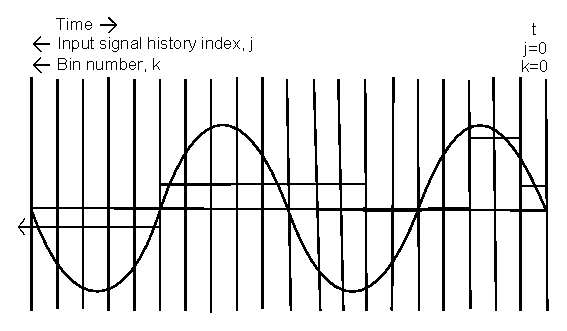
\epsfig{file=FIG1A.eps, height=40mm, width=90mm}
\\a. Higher frequency\\
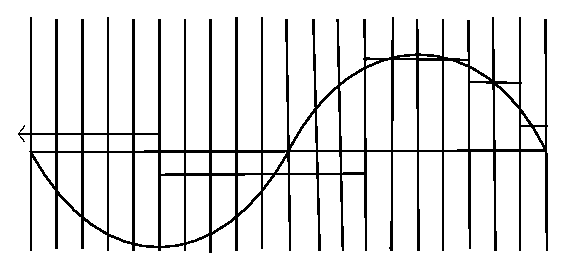
\epsfig{file=FIG1B.eps, height=40mm, width=90mm}
\\b. Lower fequency
\caption{Let each division represent a single time step and each horizontal  bar represent a bin. Larger amounts of time are included in bins with increasing time indices (further into the past). The value of the bin is the average of the input signal (the sine wave) at each time index within that bin. There exists some oldest bin that still responds sensitively to the input signal. This is bin number one (counting from zero) for Figure~a and bin number two for Figure~b. Since the time step (grid size) and binning structure are held fixed, at lower frequencies, the oldest sensitive bin moves further into the past. This illustrates the sensitivity of short bins at recent times to high frequencies and the sensitivity of long bins in the more distant past to low frequencies. This scaling relation motivates our binning strategies. All of the binning strategies used in this paper, with the exception of the straightforward truncated Gr{\"u}nwald sum, have bins that increase in duration further into the past, in order to achieve greater sensitivity at low frequencies.}
\label{fig:freqScaling}
\end{figure}

\begin{table}
Abbreviations and notation used this paper:\\
\begin{tabular}{  l@{ -- } l  p{3.0in}}
IIR & Infinite Impulse Response\\
FO & Fractional Order\\
GL &  Full Gr{\"u}nwald calculation\\
GL\# & Truncated Gr{\"u}nwald calculation to \# terms\\
LIN\# & Linear binning, \# bins\\
SQ\# &  Squared binning, \# bins\\
EXP\# & Exponential binning with a base of two, \# bins\\
FIB\#& Fibonacci binning, \# bins\\
$N_b$ & number of memory bins\\
$N_h$ & full history capacity of the algorithm\\
$N_t$ & number of data items up to time $t$\\
\end{tabular}
\end{table}

\subsection{Modified Gr{\"u}nwald}

The Gr{\"u}nwald form of the fractional derivative of order $\alpha$ can be written~\cite{OldSpan:74}

\begin{equation}
_0D^\alpha_tf(t) = \displaystyle \lim_{N_t\to\infty} \left(\frac{t}{N_t}\right)^{-\alpha}
\displaystyle\sum\limits_{j=0}^{N_t-1} w_{j}x_j
\label{simpleGrunwald}
\end{equation}
where $f(t)$ is the input signal at time $t$ and the $j$th value of the
input signal history is $x_j=f\left(t-\frac{j\Delta t}{N_t}\right)$. Note that $x_0$ is the value at the current time and increasing indices of $x$ correspond to more distant times in the past. The
$j$th Gr{\"u}nwald weight is

\begin{equation}
w_{j} = \frac{\Gamma(j-\alpha)}{\Gamma(j+1)\Gamma(-\alpha)}.
\label{wj}
\end{equation}
For the purposes of this paper, the order will be constrained $-1<\alpha<1$. Note 
that a fractional order integral is simply a derivative of negative order. Both 
derivatives and integrals are computed over a finite interval. It is assumed
that the system is non-initialized; that is there are no initial conditions.

To include more distant history at low computational cost, we modify
the Gr{\"u}nwald sum of Equation~\ref{simpleGrunwald} by partitioning its
history into $N_b$ bins. In each bin $k$, the input signal history
$x_j$ is represented by its average value over that bin, $X_k$.

Since we make the assumption that each value is well represented by
its average within a bin, we can define a value for the "bin
coefficient" by summing the Gr{\"u}nwald coefficients within that bin.

\begin{equation}
W_k = \displaystyle\sum\limits_{j=p_{k-1}+1}^{p_k} w_j
\label{eqn:sumWk}
\end{equation}

\noindent where $w_j$ is summed from the lowest index of the input data history within bin $k$ to the highest index $p_k$ within that bin. Define
\begin{equation}
N_h=p_{N_b}=\displaystyle\sum_{k=0}^{N_b}b_k,
\label{eqn:Nh}
\end{equation}
for later reference. Here $b_k$ is the number of time indices within the $k$th bin. 

With these definitions, the modified Gr{\"u}nwald differ-integral can be written

\begin{equation}
_0D^\alpha_t f(t) = \displaystyle(\Delta t)^{-\alpha}\sum\limits_{k=0}^{N_b}\bar{W}_kX_k
\label{avgSimpleGrunwald}
\end{equation}
where $\Delta t$ is the interval between time samples. There is an additional factor that goes into $\bar{W}$ that will be discussed in Section~\ref{sec:shifting}. Note that in the average Gr{\"u}nwald algorithm, $N_h$ plays the role of the last virtual time element to effectively enter the modified summation, rather than $N_t$. Here, $N_t$ plays the role of the number of time steps that have occurred since the algorithm started to run. 



\subsection{Updating the average input signal history (bin values)}
\label{sec:shifting}

As time steps forward, the input signal history $x_j$ and its binned counterpart, the average input signal history $X_k$, must change. The zeroth element always corresponds to the current time, so the origin of these histories essentially slides along the time axis as the calculation proceeds. When a new input data element is read, the values of the average input signal history ($X_k$) are updated. The new data element is transferred into bin zero through a weighted average, updating the value of the average input signal history, $X_0$, stored in the first bin. Since data elements represent values read at time steps, they should be incompressible-- when an element leaves bin zero and enters bin one, if bin one is full, another virtual element should be pushed from bin one into bin two, and so on. This process continues until a bin that is partially full or empty is reached. For an already filled bin, to update the average data stored in the $k$th bin, we take the weighted average obtained by adding one virtual element from the $(k-1)$th bin to the $b_k-1$ identical virtual elements remaining in the $k$th bin, where $b_k$ is the bin capacity. For an unfilled bin, the virtual element that has just been shifted into the bin is averaged with the $c_k$ identical virtual elements already in the bin. This process is illustrated in Figure~\ref{fig:binShifting}.

\begin{figure}
% 25.5, 90
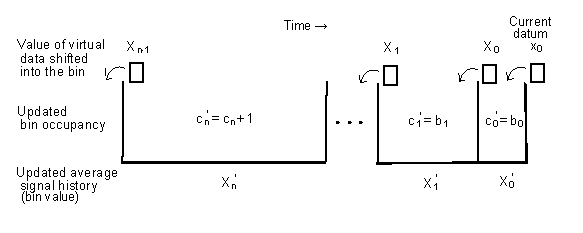
\epsfig{file=FIG2.eps,height=32mm,width=90mm}
\caption{When the input datum $x_0$ is read at the current time, virtual data elements with average input signal history values $X_k$ are shifted from the $k$th to the $(k+1)$th bin in the binned input signal history. The first $n-1$ bins are at capacity, but the $n$th bin gains one data point. The bin averages are updated to value $X_k^\prime$ through a weighted average given by Equation~\ref{eqn:updating}. At the next time step, the whole structure will step forward along along the time axis and read the next datum in the sequence, pushing back a new chain reaction of virtual data. Since bins increase in duration at higher time indices and more virtual data elements of identical values share a bin, the influence of an individual datum is diluted as it is shifted further back into memory.}
\label{fig:binShifting}
\end{figure}

During start-up, it will be necessary to consider a bin that has some
set size $b_k$, but is not filled to that capacity. In that case, it
is the current occupation number $c_k$ of that bin that enters the
calculation. The algorithm for updating bins can be stated generally if the occupation number of the $k$th bin is defined to be $c_k$. In that case, $c_k=b_k$ for all the bins more recent than the bin that is in the process of filling. No updating occurs for older bins. 

If the $k$th bin initially contains $c_k$ elements,
updating the history either leaves $c_k$ ($c_k^\prime=c_k=b_k$) or
increments the number of elements in the bin such that $c_k^\prime =
c_k + 1$ if the bin is not yet at capacity. 

Taking into account both weighted average and capacity effects, when a new virtual element is shifted into the $k$th bin, the bin's new value $X_k^\prime$ is given by 

\begin{equation}
X_k^\prime = \frac{c_k^\prime-1}{c_k^\prime}X_k + \frac{1}{c_k^\prime}X_{k-1}.
\label{eqn:updating}
\end{equation}
where $X_k$ is the old value of the $k$th bin and $X_{-1}$ is taken to be $x_0$, the input data that has just been
read. 

During start-up, the partially full bin also factors into
the Gr{\"u}nwald weights. To handle the bin that is partially full, we
weight the binned Gr{\"u}nwald weights by the ratio of the bin occupation
number $c_k$ to its capacity $b_k$,

\begin{equation}
\bar{W}_k= \frac{c_k W_k}{b_k}.
\label{eqn:Wbar}
\end{equation} 









%%%%%%%%%%%%%%%%%%%%%

\section{Computational efficiency}\label{sec:computation}
The computational efficiency of each algorithm concerns both the
memory used by the algorithm and the number of computational steps
required for the algorithm to execute, which is a measure of the
speed. To characterize the operational efficiency of a digital fractor
operating as a circuit element in real time, the quantities of
interest are the memory or number of processor steps {\em per time
  step}.

There are three phases of the computation that factor into the
computational cost of the binned Gr{\"u}nwald algorithm: initialization
(including summing the binned Gr{\"u}nwald weights), updating the average
values of the stored history in the bins as new input data is read,
and summing the modified Gr{\"u}nwald differ-integral.

During initialization, several things must happen. The array defining
the binning structure, $b_k$, must be set. The history of the input
signal must be zeroed and the first output must be set to zero. Most significantly, the binned weights must be calculated for
the chosen binning structure.

The time it takes to calculate or set $b_k$ is moderately dependent
upon the details of the binning structure chosen. However, any binning
structure will have a processing time that scales as $N_b$, the number of memory storage bins, rather than
$N_h$, the history capacity, because $N_b$ is the number of bins that must be set.

On the other hand, since each of the $N_h$ individual Gr{\"u}nwald weights
must be summed, the time for initialization of the weights scales as
$N_h$. Typical values of $N_h$ are of order $1,000$ to $10^6$. Typical
values of $N_b$ are $10$ to $26$. Since $N_h>>N_b$, the bulk of the
initialization process occurs during the computation of the weights
and the rest of the initialization process may be neglected. The time
for initialization as a whole scales as $N_h$.

By the very design of the algorithm, there is no need to store the
full Gr{\"u}nwald weights. The largest arrays that need to be stored are
the binned weights and the bin capacity, each of which has size
$N_b$. As a result, memory scales as $N_b$ rather than
$N_h$. Equation~\ref{eqn:sumWk} gives the algorithm for the calculation
of the bin weights. The following recursion formula for Gr{\"u}nwald
weights can be used to iterate $w_j$ to a new value with each time
step. In the $j$th time step, $w_j$ has the value

\begin{equation}
w_j = \frac{j-1-\alpha}{j}w_{j-1}.
\label{eqn:GrunwaldRecursion}
\end{equation}

In the implementation of an algorithm for initialization of the
weights, individual G{\"u}nwald weights $w_j$ need not be stored in an
array after calculation. These individual weights can be summed
immediately into the corresponding bin weights $W_k$ according to
Equation~\ref{eqn:sumWk}, at which time the value of $w_j$ may be
safely overwritten with $w_{j+1}$ in order to minimize the amount of
memory required such that it may be possible to later migrate the code
to an mcu.

When new input data is read, the time required to update the binned history values scales as at most $N_b$ because there are $N_b$ bins that must be
updated. Equation~\ref{eqn:updating} may be used as the basis for an
algorithm to accomplish this goal. Care must be taken to account for
the filling of the bins until the approximation reaches steady-state.

This time a memory saving  and speed enhancing opportunity is available. Since only one bin
can be filling at a time and the rest must be either full ($c_k=b_k$)
or empty ($c_k=0$), the full array of $N_b$ occupancy numbers $c_k$
need not be stored. Instead, it is sufficient to store the index of
the bin that is filling, $k_{filling}$ and its occupancy,
$c_{filling}$. These unfilled bins with $k>k_{filling}$ and $c_k=0$
are not updated when a new input signal value is read into the
history. With this approach, the algorithm becomes
\begin{equation}
X_k^\prime = \frac{c_{filling}-1}{c_{filling}}X_k + \frac{1}{c_{filling}}X_{k-1}
\label{eqn:shift1}
\end{equation}
for $k<k_{filling}$ and

\begin{equation}
X_k^\prime = \frac{b_k-1}{b_k}X_k + \frac{1}{b_k}X_{k-1}
\label{eqn:shift2}
\end{equation}
for $k=k_{filling}$ with no shift occurring for $k>k_{filling}$ since
there are no elements in those bins. Since no computation occurs for $k>k_{filling}$, the updating algorithm truly scales as $k_{filling}$ per time step, which is at most $N_b$. 

While it is possible to achieve a memory savings by storing only
$c_{filling}$ and $k_{filling}$, in the C++ code reported in this
paper, the full array of $c_{k}$ is stored. This does not impact the
memory scaling of the updating algorithm. Updating the stored bin
history values scales as $N_b$ in memory because the largest arrays
that need to be stored are the binned average values, the bin
capacity, and the bin occupancy, each of size $N_b$.

However, we do implement the speed enhancing aspect of the algorithm. In the code reported in this paper, the calculation is truncated at $k_{filling}$ rather than looping over the full $N_b$ bins to obtain the $k_{filling}$ scaling in time. 

The two real-time operation stages, updating and differ-integrating,
together require less than $400$ flops for $26$ bins of
history. For $26$ bins, less than $100$ memory registers are
required. Initialization, on the other hand, is very
resource-consuming. $N_h$ may be larger than a million and still not
fill $26$ bins. Initialization therefore may require more than a
million flops.

The binned Gr{\"u}nwald algorithm may be written in terms of either the
number of elements per bin, $b_k$, or in terms of the maximum time
step $p_k$ included within each bin (see
Equation~\ref{eqn:sumWk}). While we explain our algorithms in terms of
$b_k$ in this paper, the results derived from our C++ code were
obtained using the $p_k$ method.



%%%%%%%%%%%%%%%%%%%%%%%%%%%%%%

\section{Validation methods}\label{sec:methods}
%Methods
While the algorithms described in Section~\ref{sec:algorithmDefn} are
ultimately intended for use in a digital fractor, in order to
characterize their frequency response we have simulated them in C++ on a
personal computer. The relative phase as a function of frequency is based upon the
fractional derivative or integral of sinusoidal inputs, sweeping from
low frequency to high frequency in logarithmic steps. Relative phase
is reconstructed by curve fitting (adapted from Numerical Recipes in C~\cite{Press:92}), using the last
half of the output signal to the sine and cosine components of a
sinusoidal signal with the same frequency as the input signal. From that, phase and amplitude are calculated.

To verify phase accuracy, we examine the phase shift of a single
crossing in the time domain for an input frequency of $0.7924$ Hz
(Figures~\ref{fig:timeDomain}). Table~\ref{tab:phaseRecon}
shows a comparison of reconstructed phases using the sinusoidal fit
method and phases obtained from Figure~\ref{fig:timeDomain} by
measuring the phase difference in a single zero-crossing. The results demonstrate that the reconstructed phases are accurate when the output phase is within about ten degrees of the expected phase. Since we are interested in the deviations of the phase from the expected phase by about ten degrees, this should be sufficient. Transients may account for the remainder of the discrepancy in phase in the cases where the single crossing phase and the fit phase differ more dramatically. 


\begin{figure}
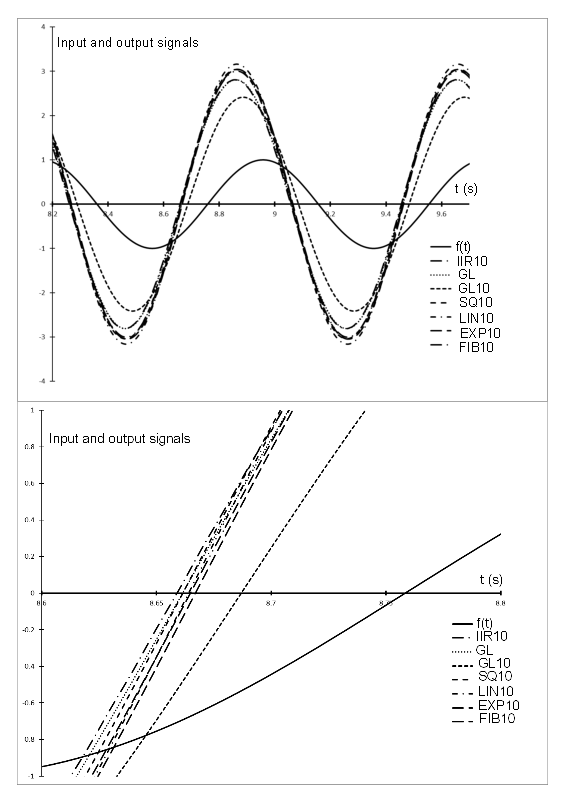
\epsfig{file=FIG3.eps, height=130mm, width = 90mm}
\caption{Zero crossings of a $0.5$ order derivative of a sine wave input signal
at long times relative to the period. From this the reconstructed
  phase can be verified using the knowledge that the frequency of this
  sine wave was $0.7924$ Hz. Reconstructed and zero-crossing phases
  are shown in Table~\ref{tab:phaseRecon}. In this plot, the duration
  was $10.0$ s and there were $1000$ time steps such that $\delta t=0.01$ s. There were 10 terms
  in the IIR and 10 bins in all binned Gr{\"u}nwald approximations. A
  variety of binning methods were used: truncated simple Gr{\"u}nwald
  (GL), linearly increasing bin sizes (LIN), bin sizes increasing as a
  square (SQ), exponentially increasing bin sizes (EXP), and bin sizes
  following a Fibonacci rule (FIB).}
\label{fig:timeDomain}
\end{figure}

\begin{table}
\begin{tabular}{llllllll}
\hline
Name &Reconstructed (degrees) &Zero-crossing (degrees)\\ IIR40 &$45.0$
&$45\pm 2$\\ GL &$44.2$ &$41\pm 2$\\ GL26 &$23.0$ &$32\pm 2$\\ LIN26
&$46.1$ &$41\pm 2$\\ SQ26 &$44.4$ &$41\pm 2$\\ EXP26 &$42.1$ &$41\pm
2$\\ FIB26 &$43.0$ &$41\pm 2$\\
\hline
\end{tabular}
\caption{Phases reconstructed through sinusoidal fits and phases approximated through single zero-crossings of a single frequency ($0.7924$ Hz) based upon Figure~\ref{fig:timeDomain}, with an expected phase of $45^\circ$.}
\label{tab:phaseRecon}
\end{table}

The simulation has successfully been run for up to $1,000,000$ time
steps, limited primarily by memory considerations due to the storage
necessary for phase and amplitude reconstruction. At this long
simulation duration, amplitudes and phases over six decades in
frequency are obtained.


%%%%%%%%%%%%

\section{Results}\label{sec:bode}

In a typical instance of the current state of the art algorithm, the
continued fraction expansion (CFE), the expansion depends upon the
last ten elements in the input signal history.{\bf CITATION} To make a
fair comparison between fractional derivative or integral algorithms,
it we examine the average Grunwald algorithm with ten bins of input
signal history, such that the history memory requirement is the
same. Figure~\ref{fig:bode10p05} contains a bode plot for a fractional
derivative of order $\alpha=0.5$ with ten history registers. Compared
to the CFE10, the average Grunwald with an exponential binning
structure (EXP10) has an approximately half a decade gain in
constant-phase bandwidth. {\bf OVERSAMPLING}

The performance of the average Grunwald algorithm improves
dramatically with a small increase in the number of input signal
history bins. The number of input signal history bins was limited by
the computational abilities of the computer for both the CFE and the
average Grunwald algorithms. For the CFE, the maximum input signal
history depth was $40$ steps into the past. For the average Grunwald,
it was possible to run up to $26$ bins ($>10^7$ steps into the past
for exponential binning). Figure~\ref{fig:bode40_26} compares the $40$
history memory registers of the CFE to the $26$ history memory
registers of the average Grunwald, for a variety of binning
strategies. At low frequencies, we see that for both fractional
derivatives and integrals there is a gain in the constant phase
bandwidth of about a decade.

\begin{figure}
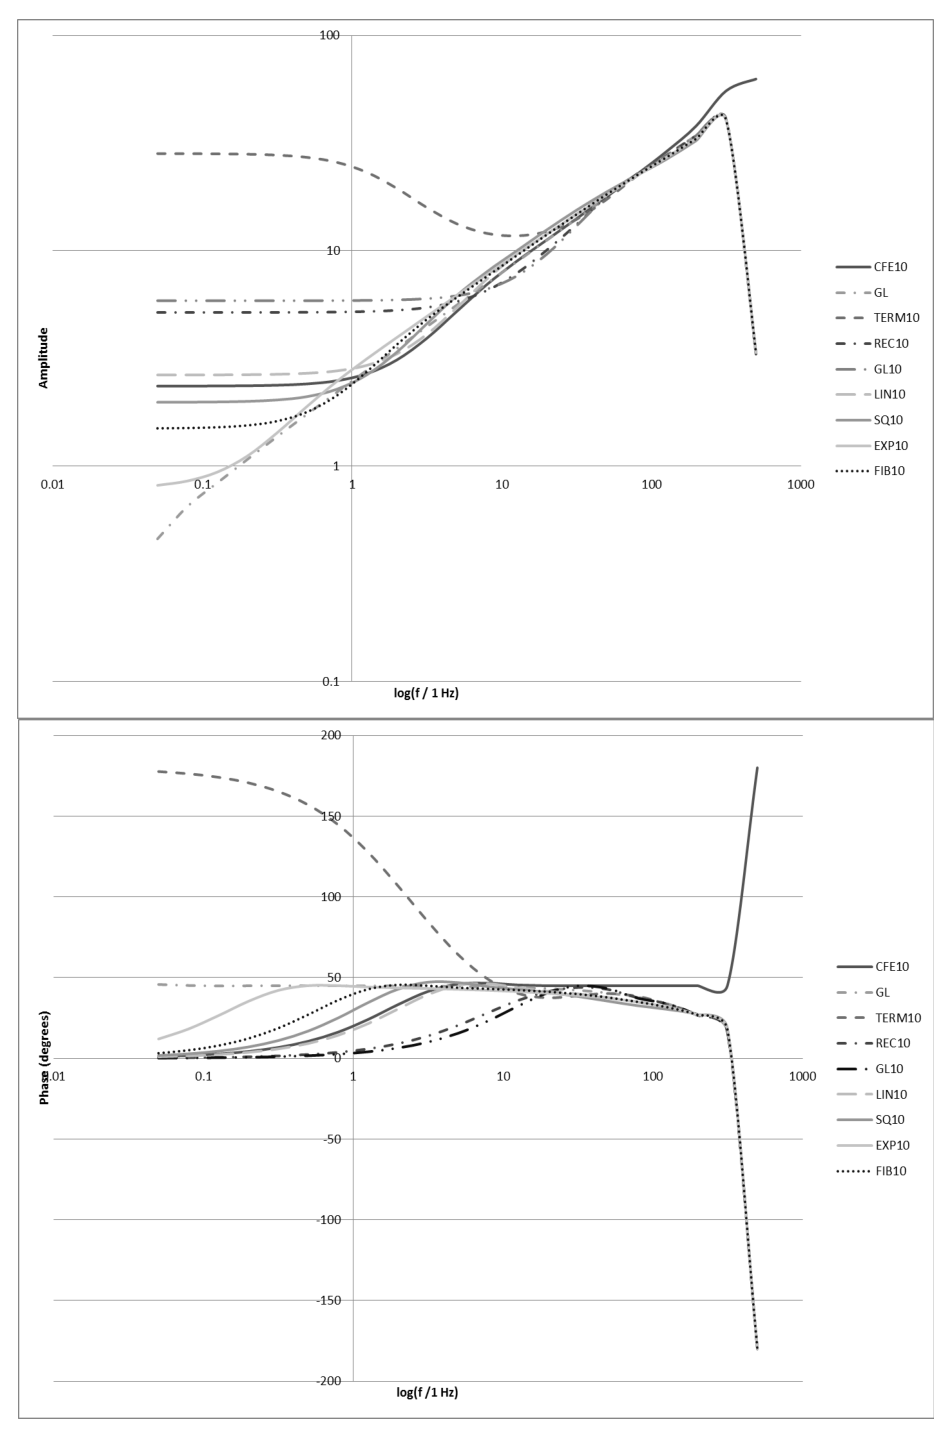
\includegraphics[width=2.5in]{bode10000_10_10_p05.eps}
\label{fig:bode10p05}
\caption{Amplitude and phase as a function of frequency for 10
  registers of binned (SQ10, EXP10, FIB10) or unbinned (GL10, CFE10)
  input signal history. GL is the full Grunwald calculation, for the
  entire input signal history prior to that time.}
\end{figure}

\begin{figure}[ht!]
\begin{center}
\subfigure{
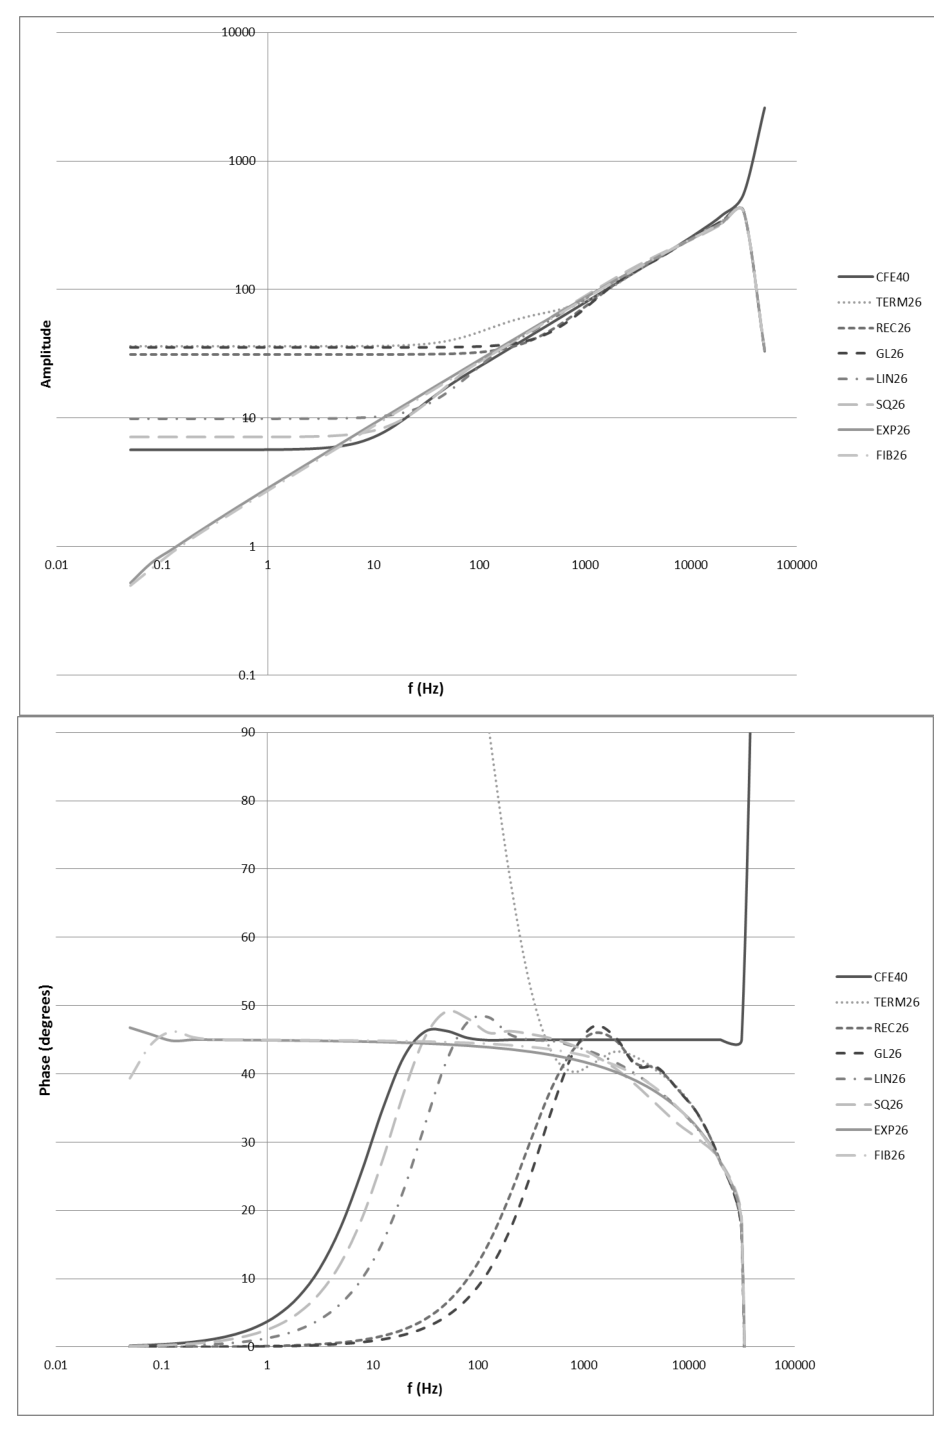
\includegraphics[width=2.5in]{bode1G_40_26_p05.eps}
}
\subfigure{
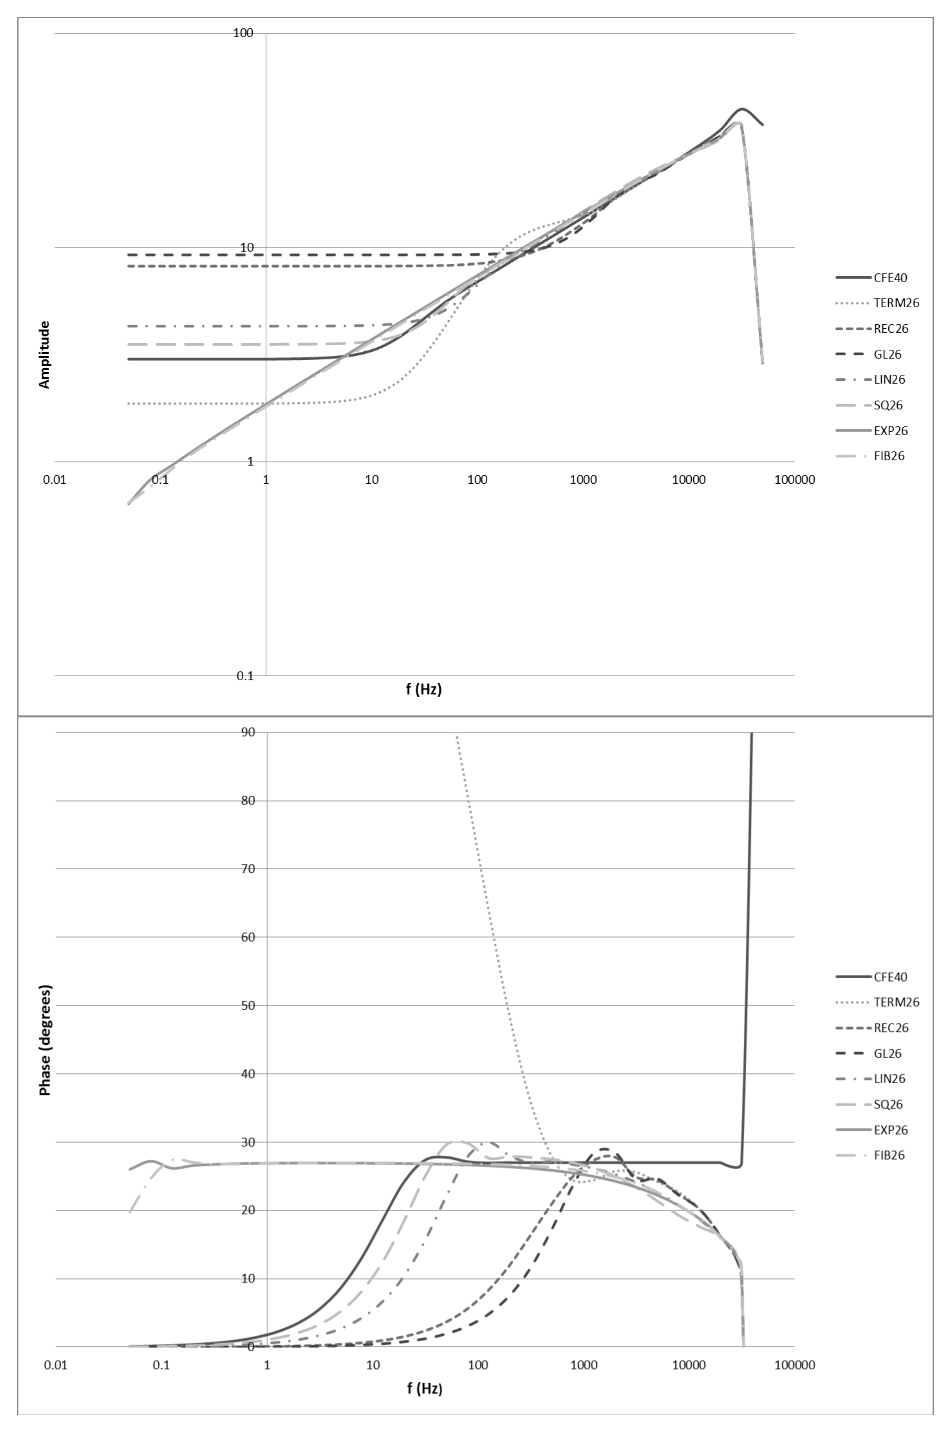
\includegraphics[width=2.5in]{bode1G_40_26_p03.eps}
}\\
\subfigure{
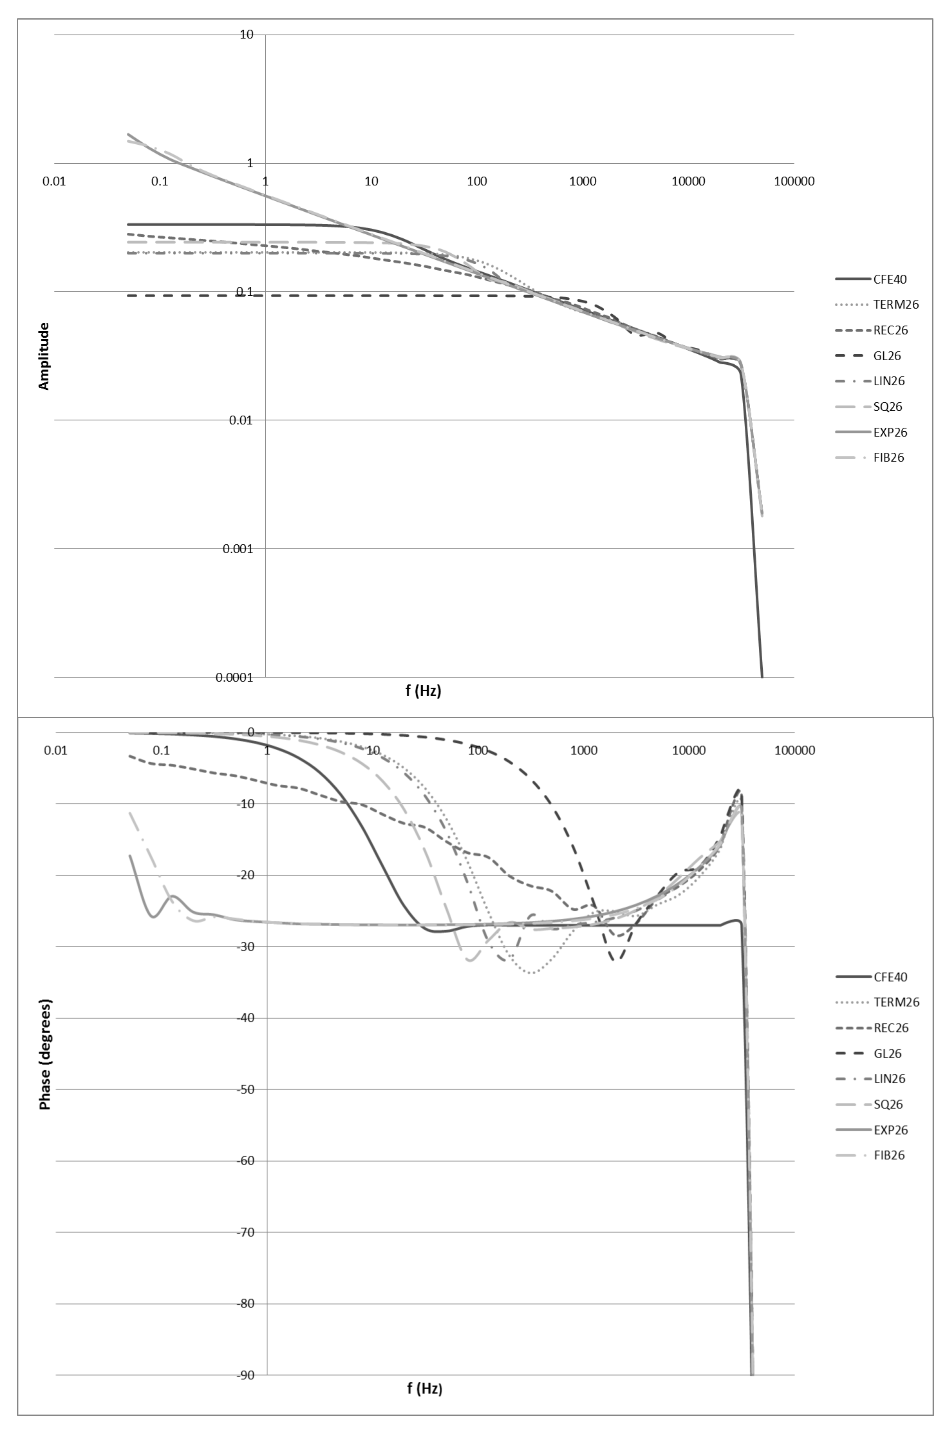
\includegraphics[width=2.5in]{bode1G_40_26_m03.eps}
}
\subfigure{
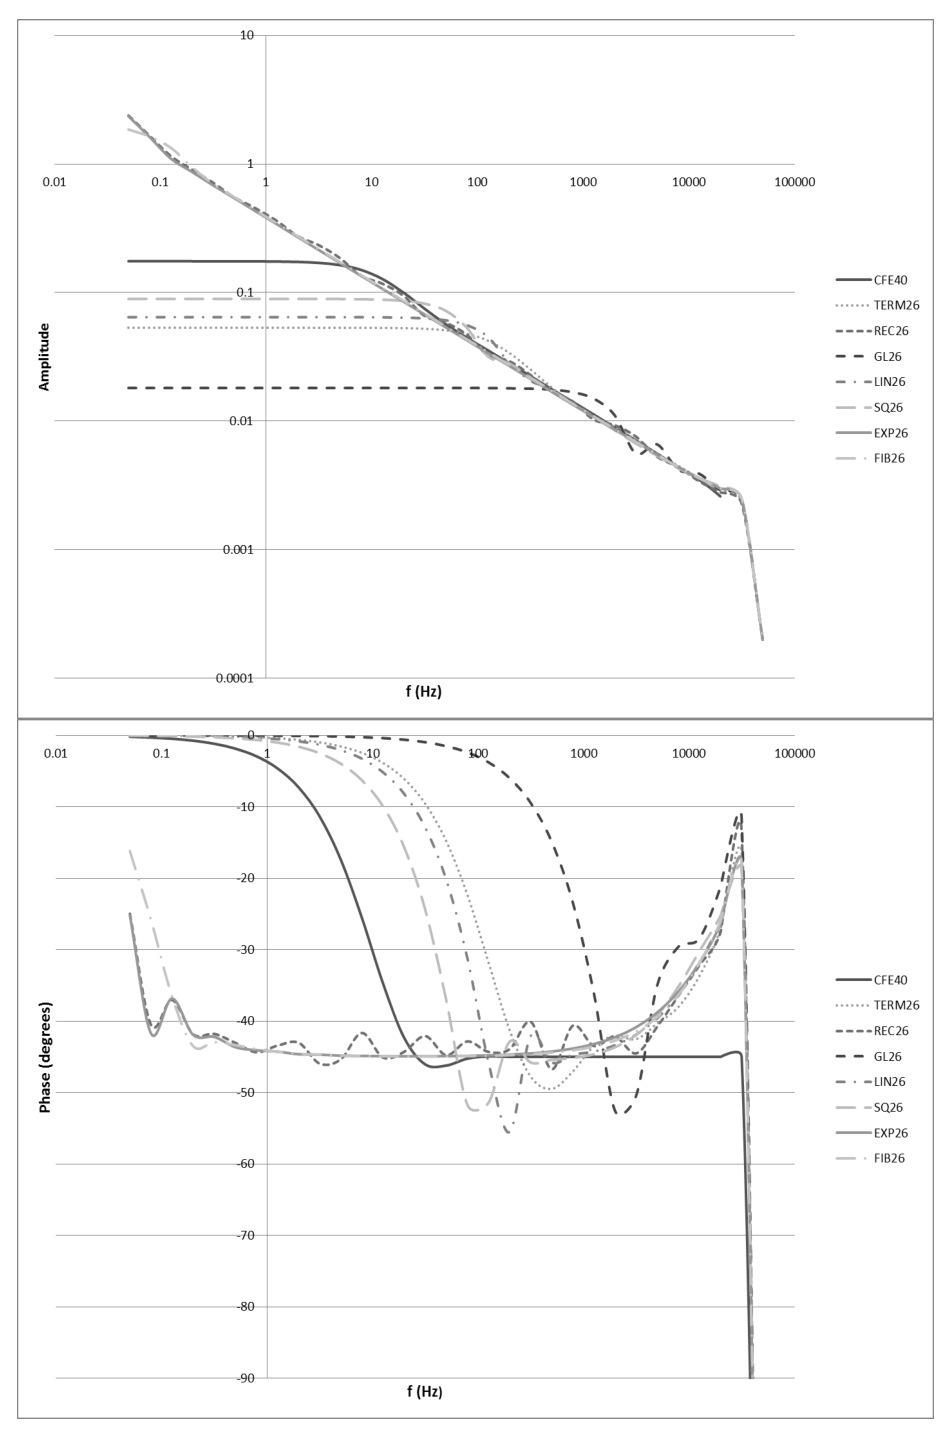
\includegraphics[width=2.5in]{bode1G_40_26_m05.eps}
}
\end{center}
\label{fig:bode40_26}
\caption{Bode plots for CFE with $40$ input signal history registers
  and average Grunwald with $26$ input signal history
  bins for $\alpha=0.5, 0.3, -0.3,$, and $-0.5$. }

\end{figure}


%%%%%%%%%%%%%%%%

\section{Conclusions}\label{conclusions}
In order to access deep memory while simultaneously conserving computational resources, we have modified the Gr{\"u}nwald algorithm by partitioning it into bins. In these bins, only the average input signal values and summed Gr{\"u}nwald weights are stored-- the individual values are discarded to conserve memory and to make the computation more efficient. We have implemented this algorithm in C++ on a desktop computer. 

Numerical simulations demonstrate that the average Gr{\"u}nwald algorithm achieves an improvement of about a factor of $3$ in constant phase bandwidth ($\pm 10^\circ$) in a fair comparison to the state-of-the-art algorithm, the Infinite Impulse Response (IIR), with its most commonly used input signal history depth (10 steps). Allowing the number of bins to be limited by the number of time steps our simulation could handle, the average Gr{\"u}nwald algorithm still makes a $2$ to $2.5$ decade constant phase bandwidth improvement over the IIR with only $20$ binned input signal history registers. 

Furthermore, during runtime, the number of flops per time step and the memory required both scale as $N_b$, the number of bins, which we have tested at $10$ to $20$. There is a one time initialization cost where the number of flops scales as $N_h$, the total number of historical time steps stored within the bins, which may be on the order of millions. Exponential binning strategies performed well at any number of bins. 

Beyond the additional bandwidth, the average Gr{\"u}nwald algorithm has a second advantage over the IIR algorithm. Commonly a low-pass filter is used to prevent aliasing. The broad roll-off  in phase of the average Gr{\"u}nwald algorithm at high frequencies would allow the Nyquist frequency to be set high when chosing an oversampling region, minimally truncating the bandwidth with the low-pass filter. Alternatively a lower order filter could be chosen, minimally disrupting the phase response. This is in contrast to the sharp plumet in phase of the IIR algorithm at high frequencies, which causes aliasing unless the highest half decade in frequency is filtered.

The ultimate goal of this work is to prepare the algorithm to be used in an mcu. Currently average Gr{\"u}nwald algorithm has been implemented as a numerical integration and differentiation package in C++. Our continuing goal will be to package it for an mcu and use it as a control element in a mechanical environment.  

%%%%%%%%%%%%%%%


%%%%%%%%%%%%%%%%%%%%%%%%%%%%%%%%%%%%%%%%%%%%%%%

%%%%%%%%%%%%%%%%%%%%%%%%%%%%%%%%%%%%%%%%%%%%%%%%%

\section*{Acknowledgments}

Thanks to Chad Bohannan for his contributions to the C++ code base and
for his thoughts on computational efficiency. The authors also thank
Saint Cloud State University for the use of computational resources.

%% The Appendices part is started with the command \appendix;
%% appendix sections are then done as normal sections
%% \appendix

%% \section{}
%% \label{}

%% References
%%
%% Following citation commands can be used in the body text:
%% Usage of \cite is as follows:
%%   \cite{key}          ==>>  [#]
%%   \cite[chap. 2]{key} ==>>  [#, chap. 2]
%%   \citet{key}         ==>>  Author [#]

%% References with bibTeX database:

\bibliographystyle{model3-num-names}
\bibliography{BohannanAbbrev}


%% Authors are advised to submit their bibtex database files. They are
%% requested to list a bibtex style file in the manuscript if they do
%% not want to use model3-num-names.bst.

%% References without bibTeX database:

% \begin{thebibliography}{00}

%% \bibitem must have the following form:
%%   \bibitem{key}...
%%

% \bibitem{}

% \end{thebibliography}
\end{document} %%%%%%%%%%%%%%%%%%%%%%%%%

